\documentclass[letterpaper, 11pt, twocolumn]{article}
\usepackage[margin=1in]{geometry}
\setlength{\columnsep}{0.75cm}

\usepackage[font=footnotesize,labelfont=bf]{caption}
\usepackage{fixltx2e}
\usepackage{tikz}
\usetikzlibrary{calc}
\usepackage{algorithm2e}
\usepackage{multirow}
\usepackage{graphicx}
\usepackage{amsmath}
\usepackage{cite}
\usepackage{framed, color}
\usepackage{color, soul}
\definecolor{shadecolor}{rgb}{.93,.93,.93}
\definecolor{blu}{rgb}{0,0,1}
\newcommand{\td}[1]{{\color{blu}\hl{TODO: #1}}}
\newcommand{\vwm}{$V_{w,n,k}$}
\newcommand{\wm}{$W_{w,n,k}$}
\usepackage{amssymb}
\usepackage{mathrsfs}
\usepackage{gensymb}

\title{Climate control for performant HPUs}
\author{}
 
\parindent0pt \parskip8pt
\begin{document}
\maketitle

\section*{Abstract}
\textbf{}
\section*{Introduction}
Although capabilities in artificial intelligence continue to advance, 
there are still many tasks for which human performance exceeds that of 
computers now and in the forseable future.  Tasks requiring repertoire of 
general knowledge about the world, the use of common sense or expert judgment, 
finding creative solutions to open-ended questions, and spontaneously 
hypothesis generation outside any apparent framework, are all examples of 
tasks that are routine for humans, but very difficult or impossible for 
computers.  The image labelling task is perhaps the canonical human 
intelligence task (HIT), perhaps because it is simply stated, nearly effortless
for humans, but still extremely challenging for computers.

Rather than replicate human intelligence, there is an alternate vision in 
which human intelligence can be freely accessed and meshed with artificial
intelligenc.  The emergence of microtask platforms like Amazon Mechanical 
Turk (AMT) has made this vision a reality to some extent.  In this paradigm,
the human processing unit (HPU) becomes one component in a hybrid 
computational system, analagous to the CPU.

But there are major challenges in building systems that deliver on this 
vision.  People are far more complex than manufactured chips, 
and so HPU performance is noisy, and subject to bias, leading to uncertain
quality of output.  Of course, the effect that HPU noise has on a compute job 
will depend on the application.
In the image labelling task, some variability is desireable, because it helps
generate sets of labels that in some sense cover semantic space occupied by an 
image.  In other cases this variability can be problematic.  In a 
transcription task, usually there is only one correct output, and so 
variability in the output only degrades quality.

Regardless of the application, the understanding HPU variance quantititively,
and the factors that influence it, will help design of efficient compute 
systems built from HPUs.

Much has been written on the factors that influence human input in 
crowdsourcing platforms.  This has generally related to the context in which
the HPU engages the task.  Unfortunately, especially for platforms like AMT,
this context is out of the designers control, and the relative anonymity of
workers makes it difficult to select for specific conditions.

In the present work, we compare influences that arise from the framing of the
task to influences that arise in-task from the mere act of working.  What 
are the effects of performance that arise simply from how the worker's 
attention is influenced by the previous task, and how do these relate 
quantititively to other pre-task influences?

We pay workers on AMT to label images, and analyze the effects brought about
by subjecting them to different priming treatments, either in the form of 
disclosing a semantically charged name of a (fictitious) organization 
funding the research, or by altering the first few images presented to the
workers.  Surpisingly, simply altering the first few images produces a much
stronger shift in subsequent labelling performance than does disclosing the 
semantically-laden name of the funder. 



\section*{Prior Work}


When considering the design of computing systems based on HPUs, we can think
of variability in HPU output as having a relatively persistent component,
and a transient one.  The persistent component would include intrinsic
qualities of a person, such as their temperament, life history, and their 
current developmental stage.  Such characteristics cannot be influenced by
the designer, but it may be possible to screen or at least characterise them 
to some extent.

The transient component of variability might include such factors as influence
alertness, orientation focus, mood, meaningfulness of the task, and any number
of aspects of mental state too subtle to describe.  Such aspects are partly
in the control of the system designer, and can be controlled through how the
task is framed and set up.

In psychology, the phenomenon of priming occurs when a prior stimulus 
makes a person more likely to respond to a task in a particular way.  The 
phenomenon is well-studied, and is believed to follow perceptual, semantic,
or conceptual similarities between the priming stimulus and the ensuing 
response.

Drawing from this insight, it is natural to wonder whether current HPU 
performance might be modulated by recently performed tasks.

Existing work on the effects of human input in crowdsourcing platforms has
generally focused on effects arising from auxilliary information, which has
been added into the task setting, or which frames the task during its 
introduction.  

For example, it was shown that framing a task in a meaningful or meaningless
way influences both task quality and the willingness of workers to produce
more output given a declining payment schedule \cite{chandler2013breaking}.
Surprisingly, relative to a zero-context treatment, although workers who were
told that there contributions would be used to help identify cancerous cells
were willing to provide more work, their work was not of a sufficiencly higher
quality.  The only effect on quality occered when workers were told that their
output would be discarded, in which case quality declined.

Another study investigated the influence of providing workers with information
about one another.  This study found that workers were willing to provide
more output, when they were able to see one another's names.  The effect was 
stronger when workers could also see some basic self-reported demographic 
information, and more still when they could see one another's responses.

In the present work, we focus on a perhaps unusual source of priming---that 
arising from the task itself, and compare this to priming that results from 
framing the work as part of study by a named organization.  Given that the 
mechanisms of priming are believed to be related to the residual activation of
perceptual, semantic, and conceptual representations, we hypothesize that 
\textit{in-task} priming could produce effects quantitively comparable to those
produced by framing.

\section*{Theoretical Framework}
Having discussed very briefly some mechanisms and cases of priming, we shall 
now seek to put forward, as an additional testable contribution, a rigorous
definition for priming that is suitable for the study of computing with HPUs.

First, we remark that it does not make sense to speak of an un-primed 
state.  When a person engages in a task, she comes to the task with some 
state of mind.  We therefore do not attempt to define priming in an absolute
sense, but rather, in a relative sense, that is, one priming can be said to 
be different from another.

Also, the effects of a given treatment will depend on the task to which the 
HPUs are put.  In other words, a treatment which generates a strong effect on
the output in one task, does not necessarily produce a strong effect on the
output for other tasks.  On a related note, the study of the effects of priming
on HPUs should be defined algorithmically.  Only effects on HPU output that
can be detected algorithmically can be relevant to a computing system built 
from HPUs.

Further, since only the influence on populations of HPU outputs can be 
meaningfully measured, and since accessing HPU power generally involves 
sampling from a pool of HPU workers, we define priming as a property of a 
population of HPU outputs.  Having said these remarks, we now present an
algorithmic definition of HPU priming:

Two populations of HPU outputs, \textsc{j} and \textsc{k}, are said to be 
\textit{differently primed} with respect to a task $\mathcal{T}$ if there 
exists an algorithm $\mathcal{A}$ which runs in time polynomial in the size
of \textsc{j} and \textsc{k}, that can distinguish 
(classify) members of \textsc{j} and \textsc{k} with accuracy 
$\frac{1+\theta}{2}$, on input \textsc{j} and \textsc{k}.  Further, $\theta$
must be a non-negligible function of $|\textsc{j} + \textsc{k}|$.
If such an $\mathcal{A}$ exists, 
we say that \textsc{j} and \textsc{k} deviate by $\theta$ in priming.

The above definition is simply intended to provide a well-defined definition
of what priming \textit{is}.  Naturally, it says nothing about the consequences
of priming.  The significance of the priming of a given population will
depend both on the nature of $\mathcal{T}$ and on the intended purpose of 
the work products derived from HPUs performing $\mathcal{T}$.


\section*{Methods}

\textbf{Task set-up.}
We paid 900 AMT workers to perform an image-labelling task.  A task consisted 
of labelling 10 images, with 5 labels each.  The first 5 images were varied 
depending on the priming treatment, while the last 5 images were the same 
accross all treatments.  Ordering of the images was kept constant.

Workers were randomly assigned to one of 6 treatments.  The treatments differed
from one another along two dimensions. The first dimension consisted of 
varying the first 5 images shown to the worker.  This was used to test the
effects of \textit{in-task} priming.

The second dimension concerned disclosure of a (fictitious) organization,
purportedly funding work as part of a research study.  Depending on the 
treatment, one of two funding agencies was presented, or no indication was 
made.

Tasks were presented to workers as a series of panels or flash cards.  The
first panel provided brief instructions, and was identical for all treatments.
Workers could see this panel when previewing the task, but could not advance.
Depending on the treatment, the worker was either shown a second pannel 
stating the name of 
one of two fictitious organizations funding the work, or this panel was 
skipped.  The next five pannels each consisting of a priming sub-tasks, 
wherein the worker was asked to submit five descriptive labels.  The images
used during the priming sub-task depended on the treatment.  The last 5 pannels
consisted of testing subtasks, wherein, as for the priming sub-tasks, workers
were asked to submit 5 descriptive labels.

\textbf{Choice of images.}
The 5 test images, were chosen with two ideals in mind.  
First, we chose images that we judged would generate a diverse vocabulary of 
labels, such that the effects of priming could be detected.  In other words,
sparse images with a single object in the foreground were not considered good 
candidates, since they would be less likely to elicit labels that varied from 
one worker and one priming treatment to the next.

Second, we chose images which would produce labels belonging to two broad
concepts, which would serve as the targets of our priming: food and culture.  
This created the opportunity to attempt to prime workers in a way that would
bias them toward emitting food-related or culture-related labels.

Under these considerations, we chose the images shown in 
Fig.~\ref{fig:testImages}.  Each of these images has food as its main focus,
but also has a strong and specific cultural reference due to the unique, 
iconic character of the food and the artifacts depicted.

To investigate in-task priming, we chose a set of images that highly
recognizeable cultural settings and no food, and another set that contained
separated food ingredients, without any overt cultural content.  The third
set of images was chosen to be very much like the test images, showing prepared
meals, and though prepared food is inseperable from culture, these images
were chosen based on being culturally more muted or ambiguous. 

\textbf{Label ontology.}
In order to provide a deeper analysis, we built an ontology
of the corpus of all labels applied to the first test image.  The ontology
was built as a directed acyclic graph starting 

\section*{Results and discussion}

\begin{figure*}
	\begin{center}
		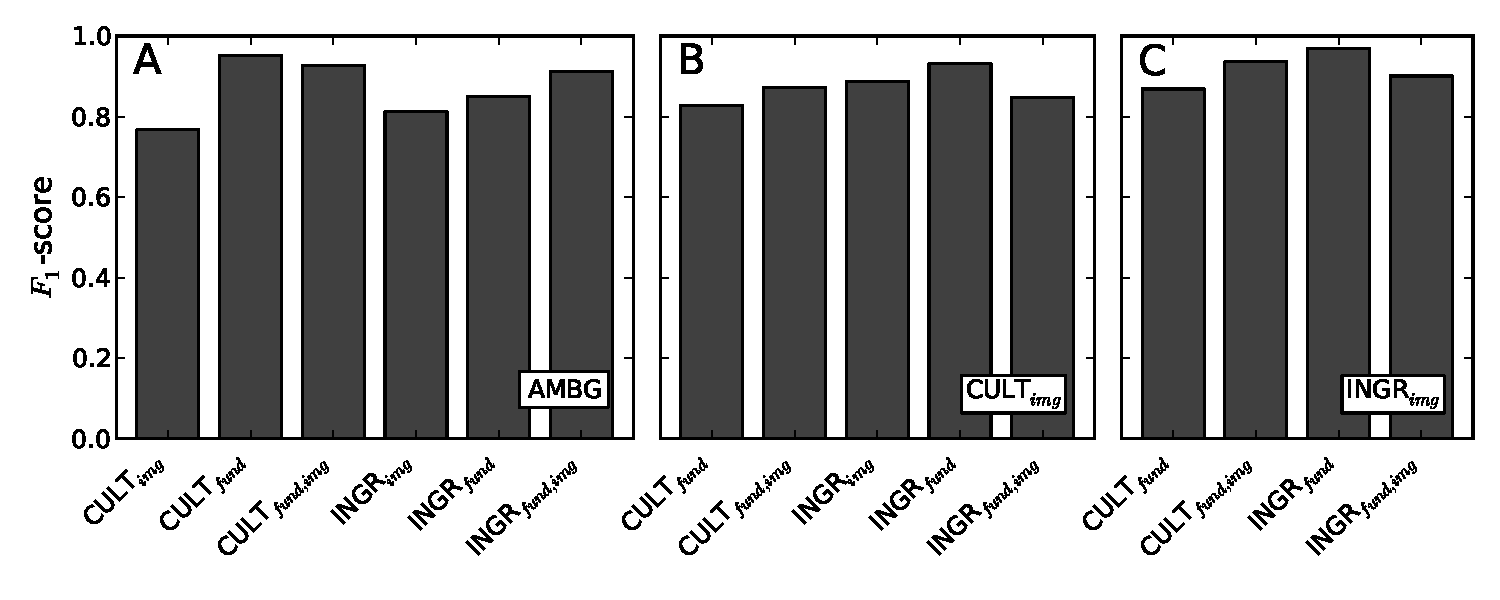
\includegraphics[scale=0.55]{../figs/f1scores.pdf}
		\caption{$F_1$-score for binary classification of HPUs from seperate
			treatments using a naive Bayes classifier.  Each pannel shows
			the performance of the classifier when distinguishing between 
			a basis treatment (inset) and the treatments listed on the 
			abscissa.
		}
		\label{fig:classifier}
	\end{center}
\end{figure*}

\textbf{Priming affects HPU output.}
Before looking for differences in the content of labels provided by workers
from different treatments, we first demonstrate that the treatments are
distringuishable in an algorithmic sense.

Using a naive bayes classifier, we are able to distinguish with high precision
and specificity between workers from the \textsc{ambg} treatment and any of
the other 5 treatments.  Fig~\ref{fig:classifier}A shows F1-score for a
naive bayes classifier when distinguishing between the \textsc{ambg} and 
the other treatments. The classifier achieves high precision and specificity
in task.  Figure~\ref{fig:classifier}B shows the F1-score for binary
classification between the $\textsc{cult}_{img}$ and the other treatments, 
while \ref{fig:classifier}C shows that for $\textsc{ingr}_{img}$ and the other
treatments.  

Not surprisingly, pairs of treatments in which one primes for culture, and the
other primes for ingredients are easily distinguished.  However, it is quite
surprising that high accuracy is achieved when classifying treatments within 
the same orientation (e.g. cultural).  This is especially true in such cases as
the classification of  $\textsc{cult}_{img}$ and $\textsc{cult}_{fund,img}$
($\text{F}_1 = 0.863$), where both treatments also share the priming images in 
common.

We find it remarkable that, using only the labels that workers provide, it is
possible to infer with good accuracy (at least when given a choice between 
two posibilities)  the treatment to which the worker was 
subjected.


\begin{figure}
	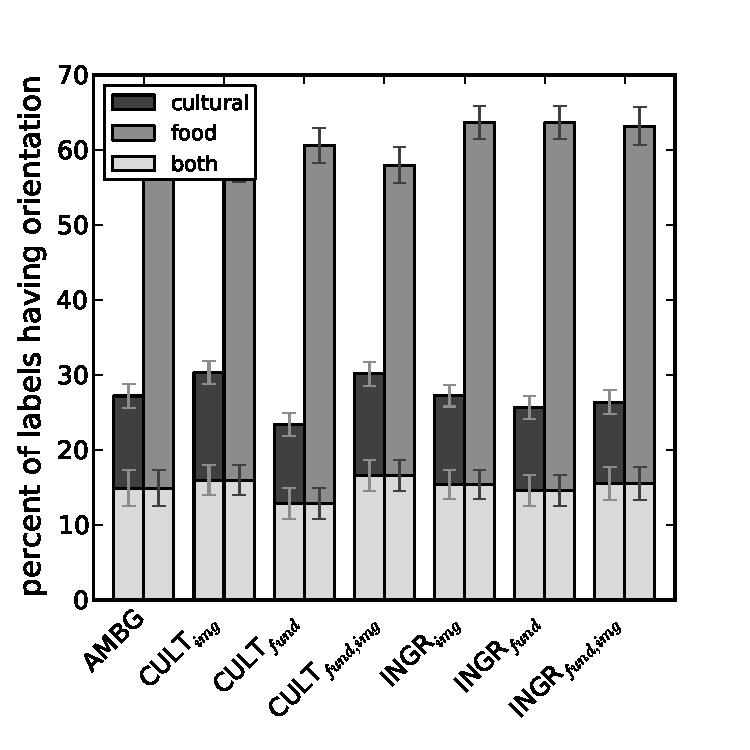
\includegraphics[scale=0.65]{../figs/valenceComparison.pdf}
	\caption{Percentage of labels of a food- or cultural- orientation, or
	both.  In our ontology of labels, a label can have multiple parents. 
	For example \texttt{naan} inherits from both \texttt{food} and 
	\texttt{cultural} through its parent \texttt{indian food}.}
	\label{fig:valence}
\end{figure}


\textbf{Priming orients HPU focus.}
Having established that each treatment does in fact consist of distinguishable 
populations of the HPUs, we next look at the content of labels.  Two of the
root labels in our ontology, \texttt{food} and \texttt{cultural}, map naturally
onto the two concepts that laid behind the design of our priming treatments.
A natural and straightforward expectation is that HPUs from treatments 
$\textsc{cult}_x$ should emit more labels that are ontological descendents of
\texttt{cultural}, while those from the $\textsc{ingr}_x$ treatments should
emit more labels under $\texttt{food}$.

In Fig.~\ref{fig:valence}, we exhibit the percentage of labels having a 
cultural orientation (i.e. descending from \texttt{cultural} in the ontology), and 
the percentage having a food orientation. Before making comparisons using this
information, we remark that there is no reason to expect a balance in the 
number of words having cultural or food orientation overall.  The $\textsc{ambg}$
treatment, which was designed to promote neither orientation, exhibits a
significant fraction of words from both the food and cultural orientation, while
significantly favoring the former.  

Both $\textsc{cult}_{img}$ and $\textsc{cult}_{fund,img}$ show a significant
excess of culturally-oriented labels and fewer food-orientel labels.  
Furthermore, HPUs in these treatments emit more culturally-oriented labels 
even while emitting fewer labes that are simultaneously oriented toward 
cultural and food (light bars in Fig.~\ref{fig:valence}).
The deviation of these treatments from
the others is well beyond the 95\% confidence interval.

Interestingly, the $\textsc{cult}_{fund}$ treatment did not have this effect.
Although we have demonstrated that $\textsc{cult}_{fund}$ is differently
primed from \textsc{ambg} using a naive bayes classifier, in respect of 
overal fraction of food- and culturally-oriented labels, no distinction 
is to be made.

In the case of $\textsc{ingr}_x$ treatments one expects to see an 
enrichment of food-oriented labels. There is perhaps some evidence for this
$\textsc{ingr}_{fund}$ and $\textsc{ingr}_{fund,img}$, but we cannat make any
assertion with confidence.


\begin{figure*}
	\begin{center}
	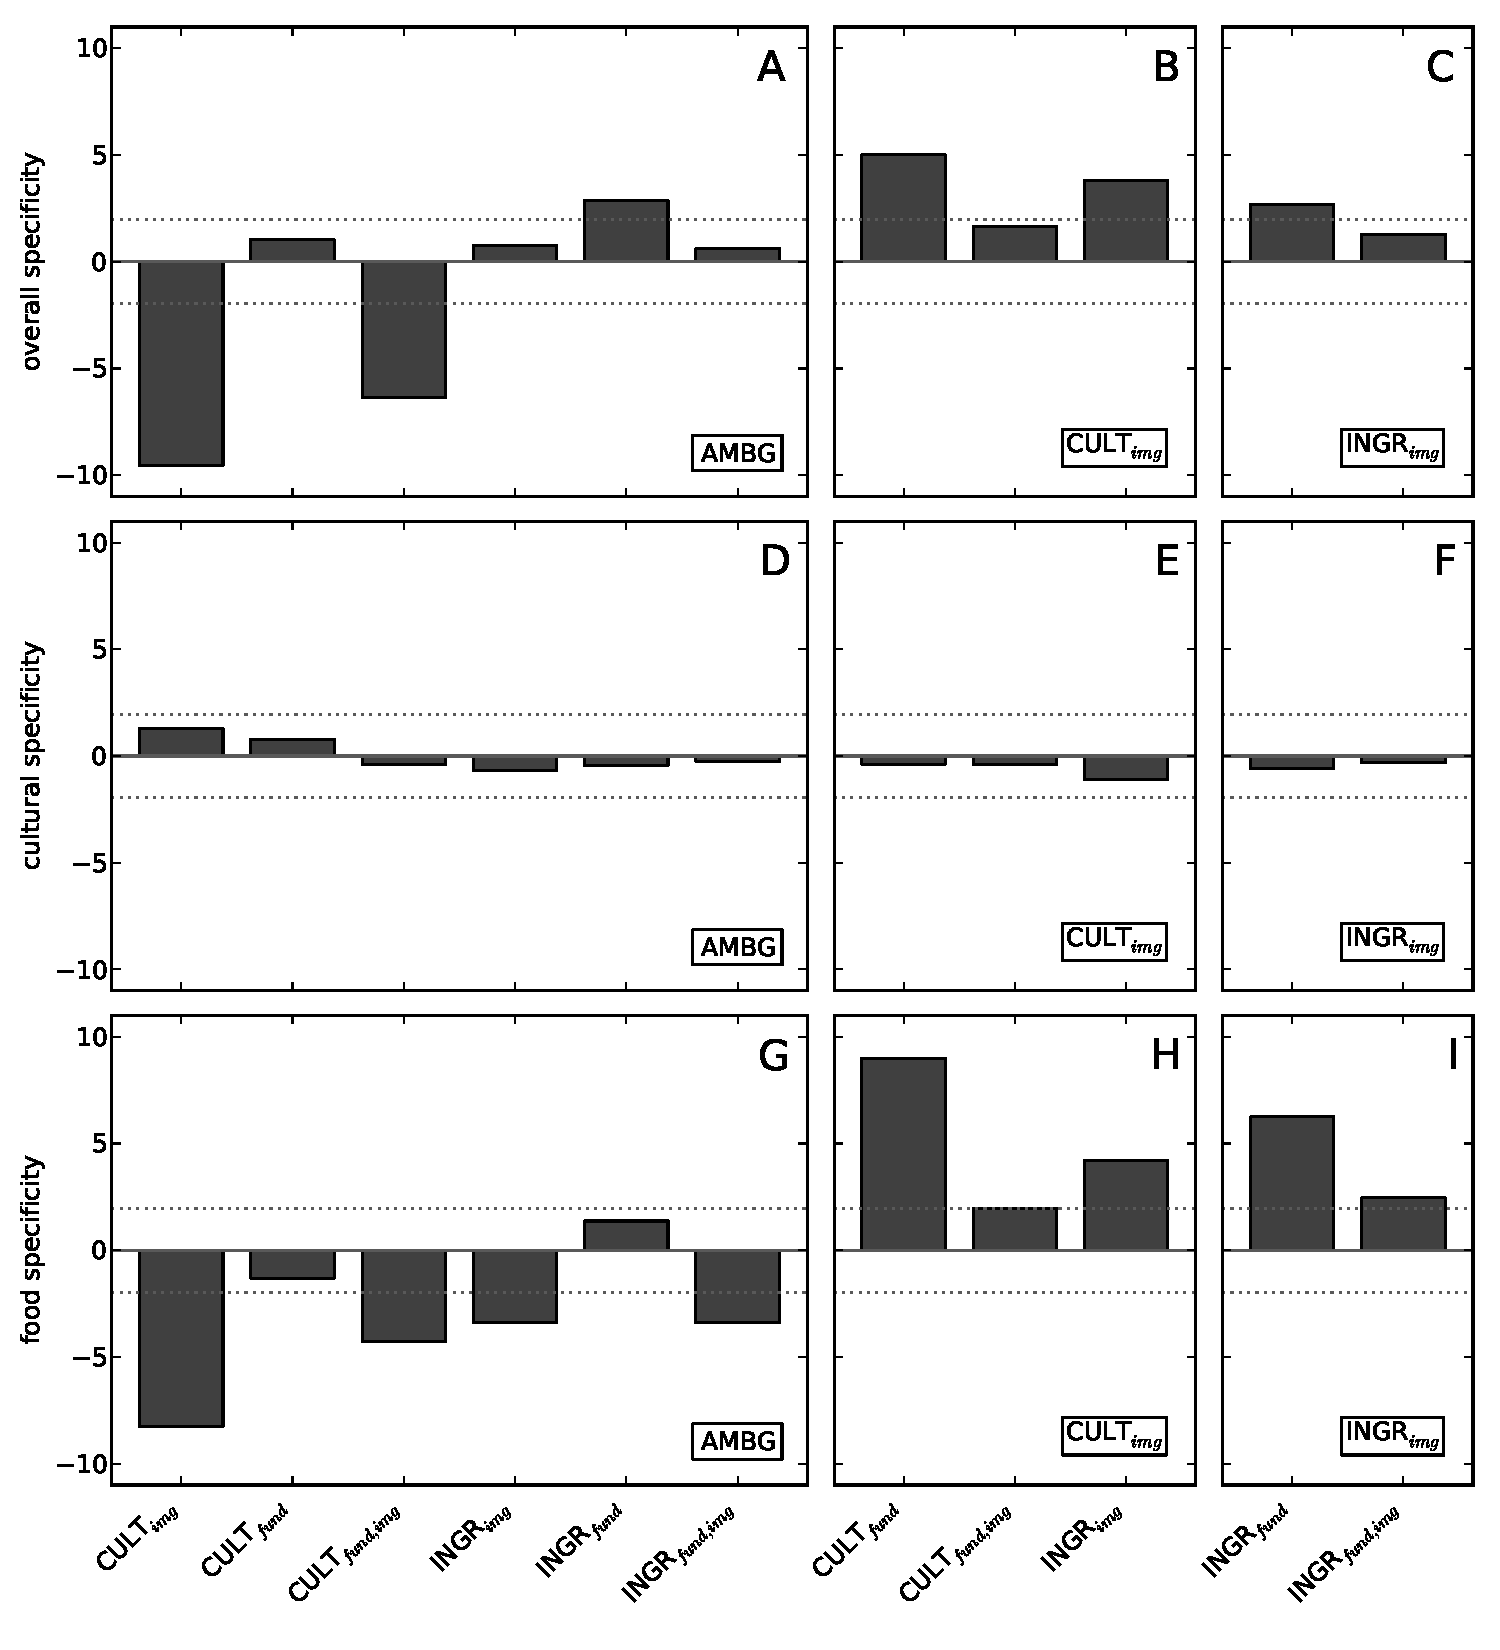
\includegraphics[scale=0.55]{../figs/specificity2.pdf}
	\caption{Pairwise comparisons of label specificity between different 
	HPU treatments.  Each pannel presents a binary comparison between a 
	basis treatment (inset) and the subject treatments indicated on the 
	abscissa.  A positive specificity score indicates that the subject 
	treatment emitted more specific words than the basis treatment overall.
	In a given comparison, a sample of 50 HPUs from the   
	each treatment was randomly sampled, and the specificity of labels from
	the HPUs of oposing treatments were compared.
	To compare two HPUs, each pair of labels from different HPUs are compared.
	and the specificity score of subject HPU is the number of cases where its
	label is more specific than the subject HPUs, less the number of cases 
	where it is more general. This score is 
	avereaged for all HPU pairings.  Statistical significance is guaged
	by generating a null-comparison between two mutually exclusive subsamples 
	from the basis treatment.  This null-comparison yields a distribution
	of relative specificities whose mean is in principle zero.  The 
	specificity scores are expressed in terms of standard deviations of
	the null-comparison specificities.  
	The dotted lines represent the 95\% confidence interval for rejecting 
	the null Hypothesis that the basis treatment and subject treatment are
	equally specific.
	}
	\label{fig:specificity}
	\end{center}
\end{figure*}

\textbf{Priming affects attention to detail.}
We next look at how alternately treated HPUs differ in their tendency to use
more specific or more general labels. We use the ontology of labels emitted
on the first test image to unambiguously establish a partial ordering of 
label-specificity.  If one label $\ell_1$ is within the ancestry of another
$\ell_2$, we say that $\ell_1$ is more general than $\ell_2$, otherwise they
are not comparable.  Thus, the label \texttt{naan} is more 
specific than both \texttt{bread} and \texttt{indian}, while uncomparable to
\texttt{statue}.

Label-specificity only generates a partial ordering---at least in our 
experimental design.  A consequence of this is that it is not possible to
assign an overall specificity score to a set of labels.  We submit that this
reflects the underlying complexity of natural language semantics.  While
we admit that there may be many ways to generate full orderings based on some
notion of label specificity, we believe that this would inappropriately 
collapse qualitative differences between labels, leading to results that are
difficult to interpret.

In Fig.~\ref{fig:specificity}, We show pairwise specificity comparisons 
between various pairs of treatments.  Figure~\ref{fig:specificity}A shows
the comparison of \textsc{ambg} with all other treatments.  Both treatments
primed with cultural images ($\textsc{cult}_{img}$ and 
$\textsc{cult}_{fund, img}$) exhibit an excess of more general words compared
to \textsc{ambg}.  Meanwhile, $\textsc{ingr}_{fund}$ emitted an excess of 
more specific words.

We can seek to explain these observations by restricting the comparison to
labels of a specific orientation (e.g. food or cultural).  When we perform
the same comparisons but restricting to food-oriented labels, as shown in 
Fig.~\ref{fig:specificity}G, we see some of the same tendencies as in A.
However, when restricting to culturally-oriented labels 
(Fig~\ref{fig:specificity}D) there are no significant comparative deviations 
in specificity to speak of.

A first conclusion that we can draw from this is that there is a significant
loss of specificity in labels emitted by treatments having non-ambiguous 
priming images.  In Fig.~\ref{fig:specificity}G, only $\textsc{cult}_{fund}$
and $\textsc{ingr}_{fund}$ show no significant deviation.  

- through negative priming workers stop responding to generic features of images of prepared meals, which happens in the ambiguous case.

- On the other hand, workers presented with either the cultural or ingredients images are initially struck by the gross differences, which draws generic 
labels, especially with respect to food for which generic labels in ambiguous treatment had been suppressed through negative priming.

- it seems, at first, inconsistent that $\textsc{cult}_{img}$ and 
$\textsc{cult}_{fund,img}$ would at once enrich the fraction of 
culturally-oriented words, but produce no change in the specificity of 
culturally oriented words.  First of all, there is no logical incompatibility
with producing a greater number of cultural terms, yet which are generic 
in nature.  If we follow the hypothesis that focus (or orientation) is directed
by positive priming (perhaps through the subconscious or conscious inference
of reqeuster intent), while focusing on nuances comes from the inhibition
of gross features through negative priming, then this combination of observations makes sense.  Having seen many cultural images, HPUs in 
$\textsc{cult}_{img}$ and $\textsc{cult}_{fund,img}$ are primed to emit 
cultural labels, however, since the diversity of images is high compared to
other treatments on reaching the test images, there no opportunity for 
focussing in to finer detail through the mechanism of negative priming.

\textbf{In-task priming is stronger than framing.}
Our experimental set-up includes two priming mechanisms: in-task priming, 
produced by varying the first 5 images of the task, as well as what could be
called sidestream priming, in which a fictitious funder is disclosed.
The intention behind this set-up was to enable a direct comparison, and 
our expectation was that in-task priming might produce some fraction of the
effect produced by disclosing the funder.  To our surprise, in-task priming 
produces a much stronger effect.

There is a cautionary lesson here.  In-task priming, which is inherently 
impossible to eliminate is may be far more severe than the more overt causes 
of priming that more routinely attract concern during the design of an 
experiment.   Depending on the final purpos of HPU work products, this may be
quite restrictive.

\textbf{Leveraging priming.}
In a more positive view, the results of our study suggest that the ordering 
of subtasks can be used as a way to direct the focus and attention to detail
by HPUs.  If the designer desires more coarse-grained work-products, this
can be achieved by presenting successive subtasks with high diversity.  On 
the other hand if fine-grained work products are desired, then the designer
should aim to sort subtasks into ``tracks'' that are highly homogeneous,
and assign subsens of the pool of HPUs to specifict tracks.

It is interesting to consider to what extent the output of HPUs can be driven
toward nuanced detail using this technique.  Consider, for example, the 
image labelling platform called the ESP Game.  Here Two HPUs are shown
the same image and in order to derive what are in some sense the moset 
characteristic labels, they are asked to attempt to produce the same labels
for the image.  One could imagine a similar setup, but in which the designer
attempts to produce the set of labels that best covers the semantic space 
occupied by the image, by eliciting labels at coarser and finer levels of 
specificity using the techniques suggested by the present work.

\begin{figure}
	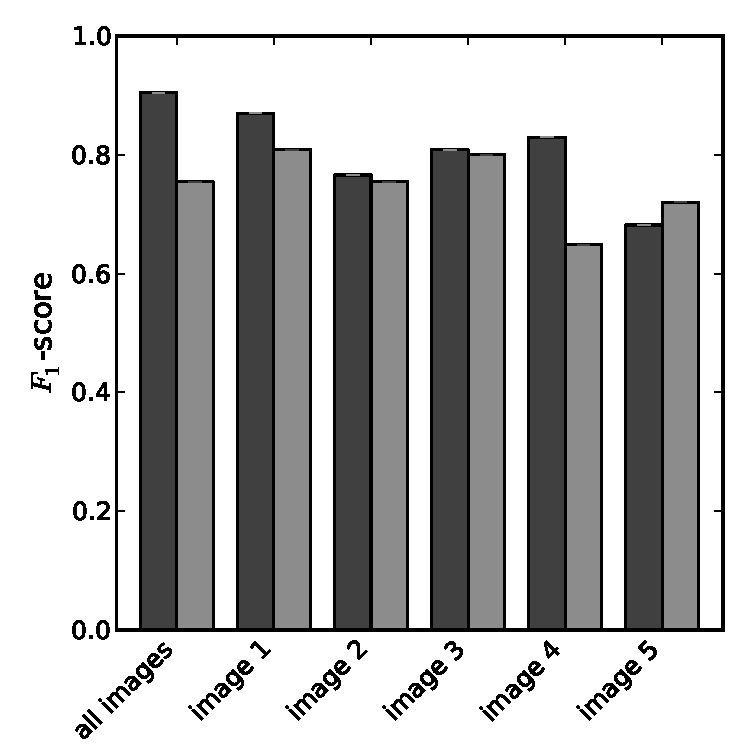
\includegraphics[scale=0.58]{../figs/longitudinalF1scores.pdf}
\caption{$F_1$-score for a naive Bayes classifier trained to distinguish
	HPUs from $\textsc{ingr}_{img}$ and $\textsc{cult}_{img}$ based on 80  
	instances from each treatment, and tested using 20 instances.  Here we
	present the performance of the classifier when only the labels from 
	specific images are presented, to exhibit whether its performance degrades 
	as the number of subtasks since priming increases. 
	}
	\label{fig:longitude}
\end{figure}


One interesting test of this hypothesis arises in 
% Graphics commented out because they make compiling take long!  
% Uncomment when desired!
\begin{figure*}
%	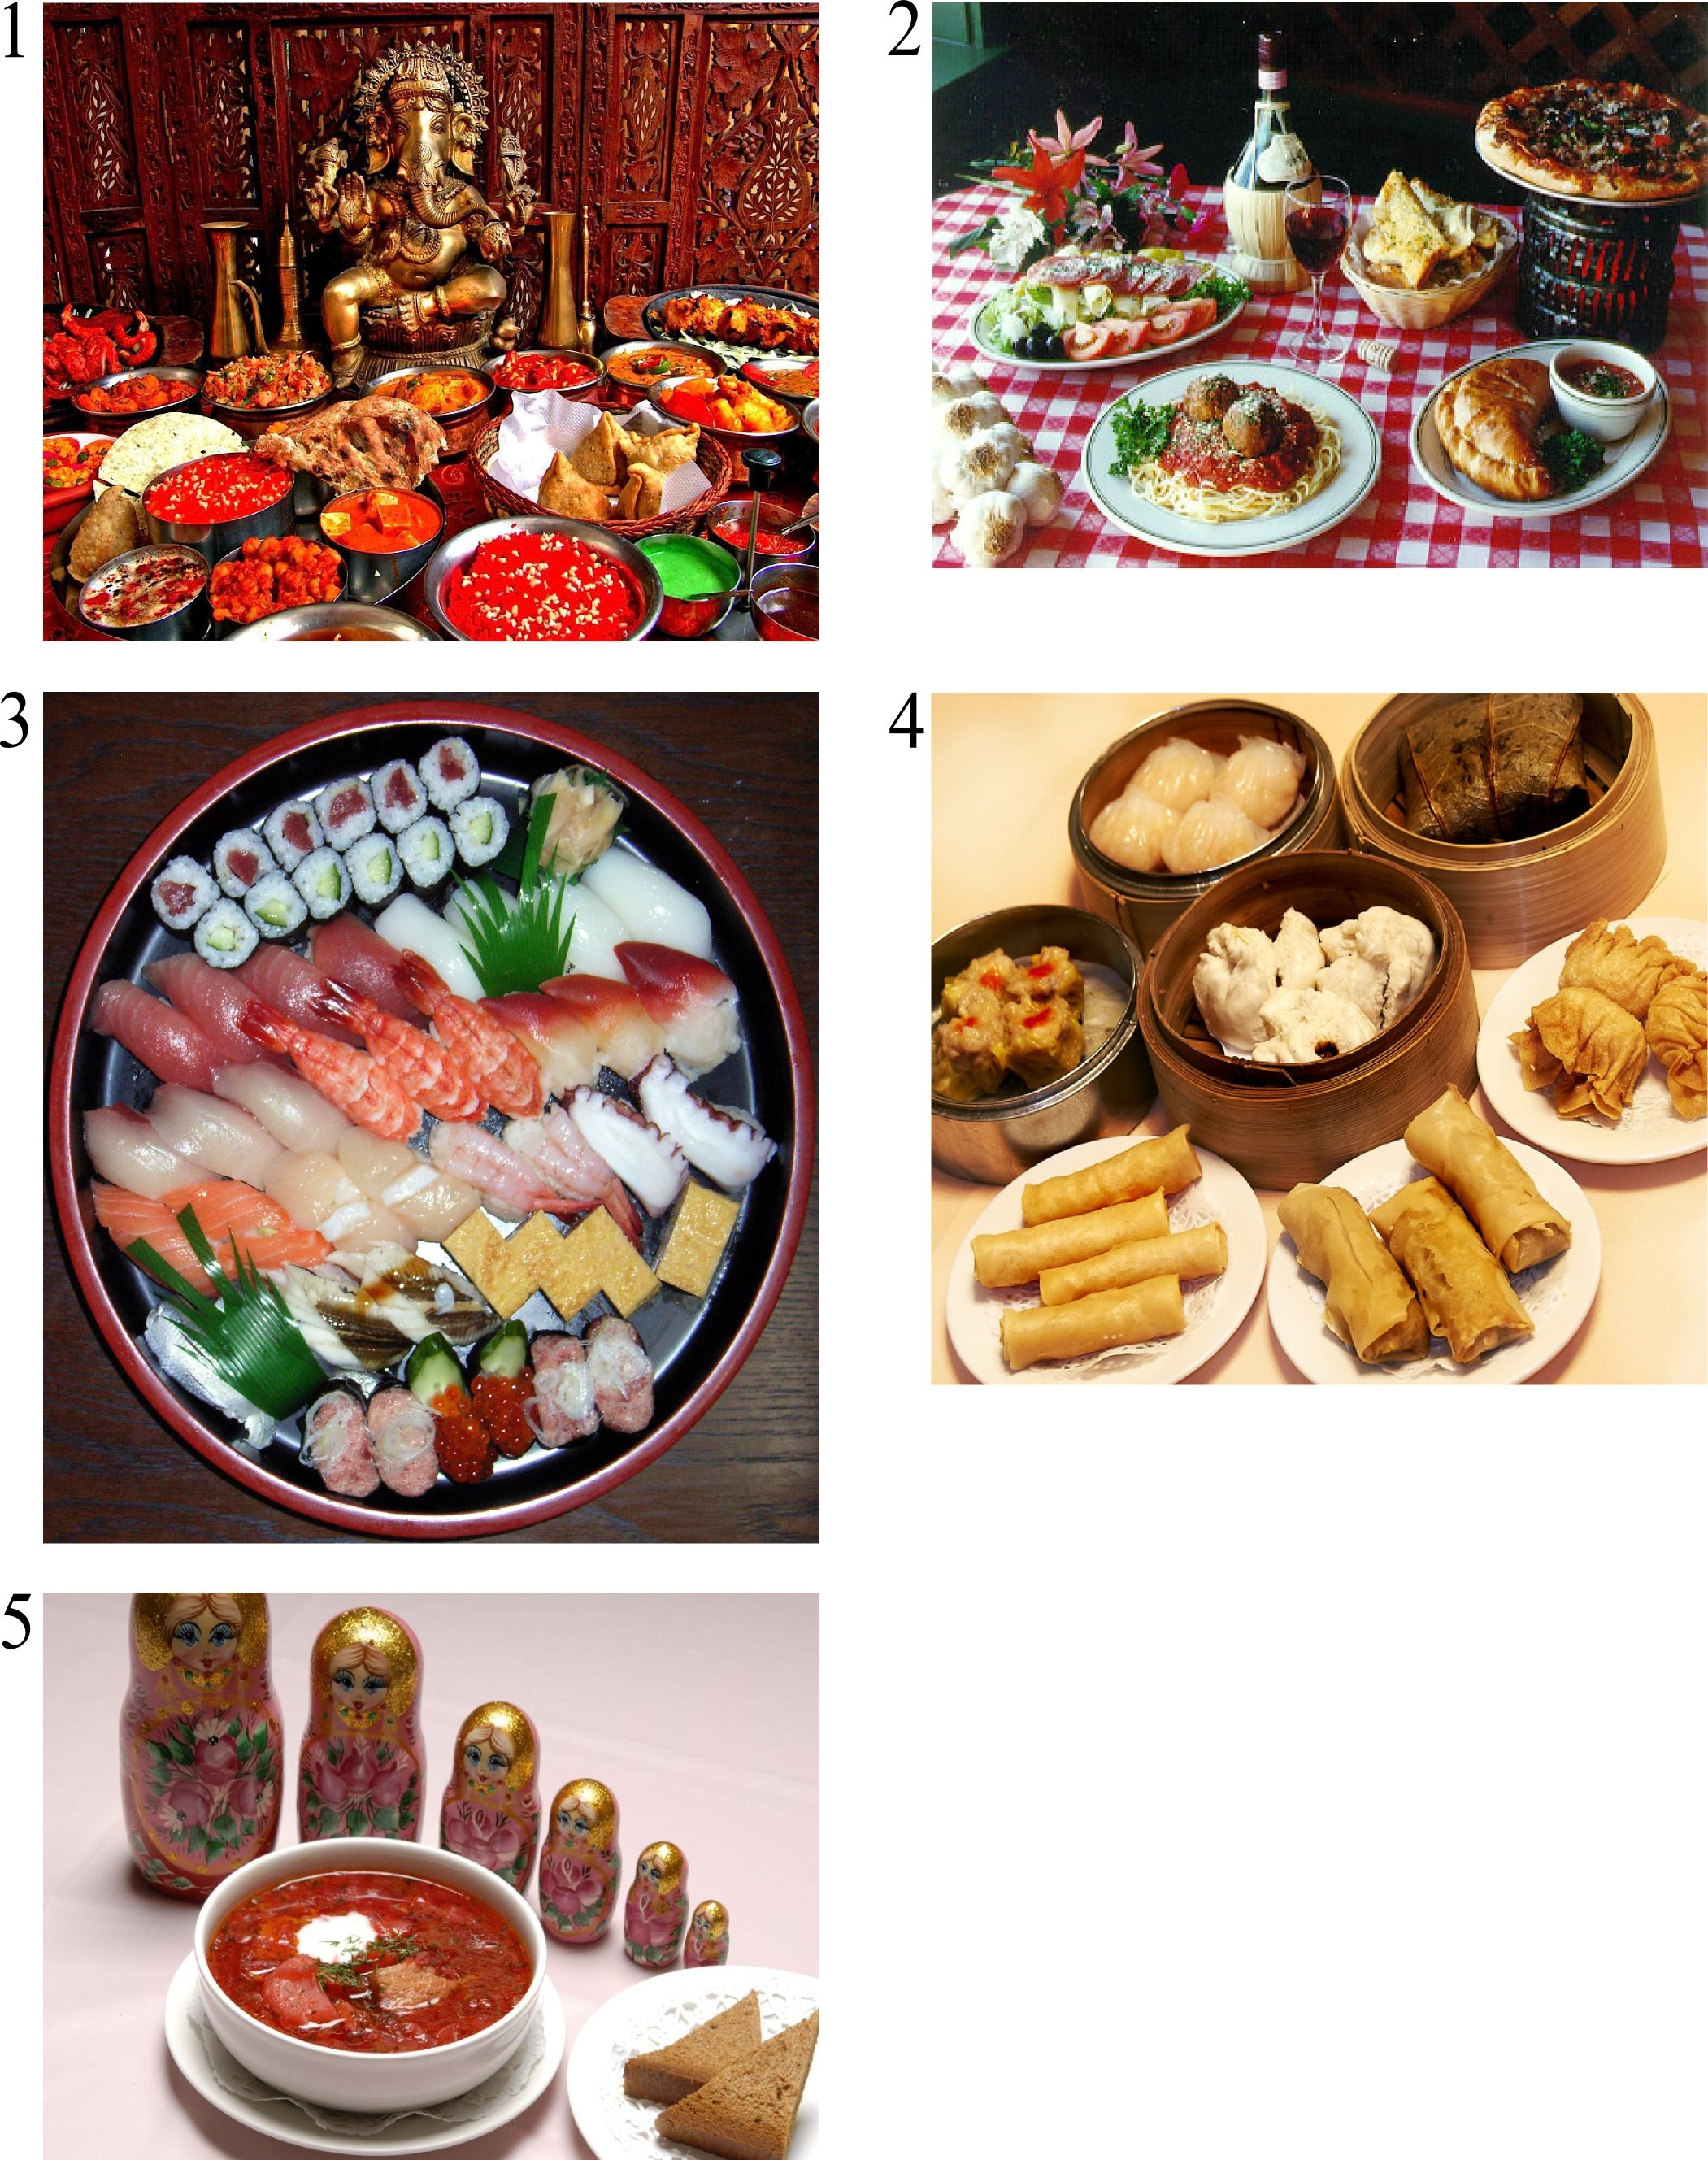
\includegraphics[scale=1.00]{../figs/testImages.png}
	\caption{caption here}
	\label{fig:testImages}
\end{figure*}

\begin{figure*}
%	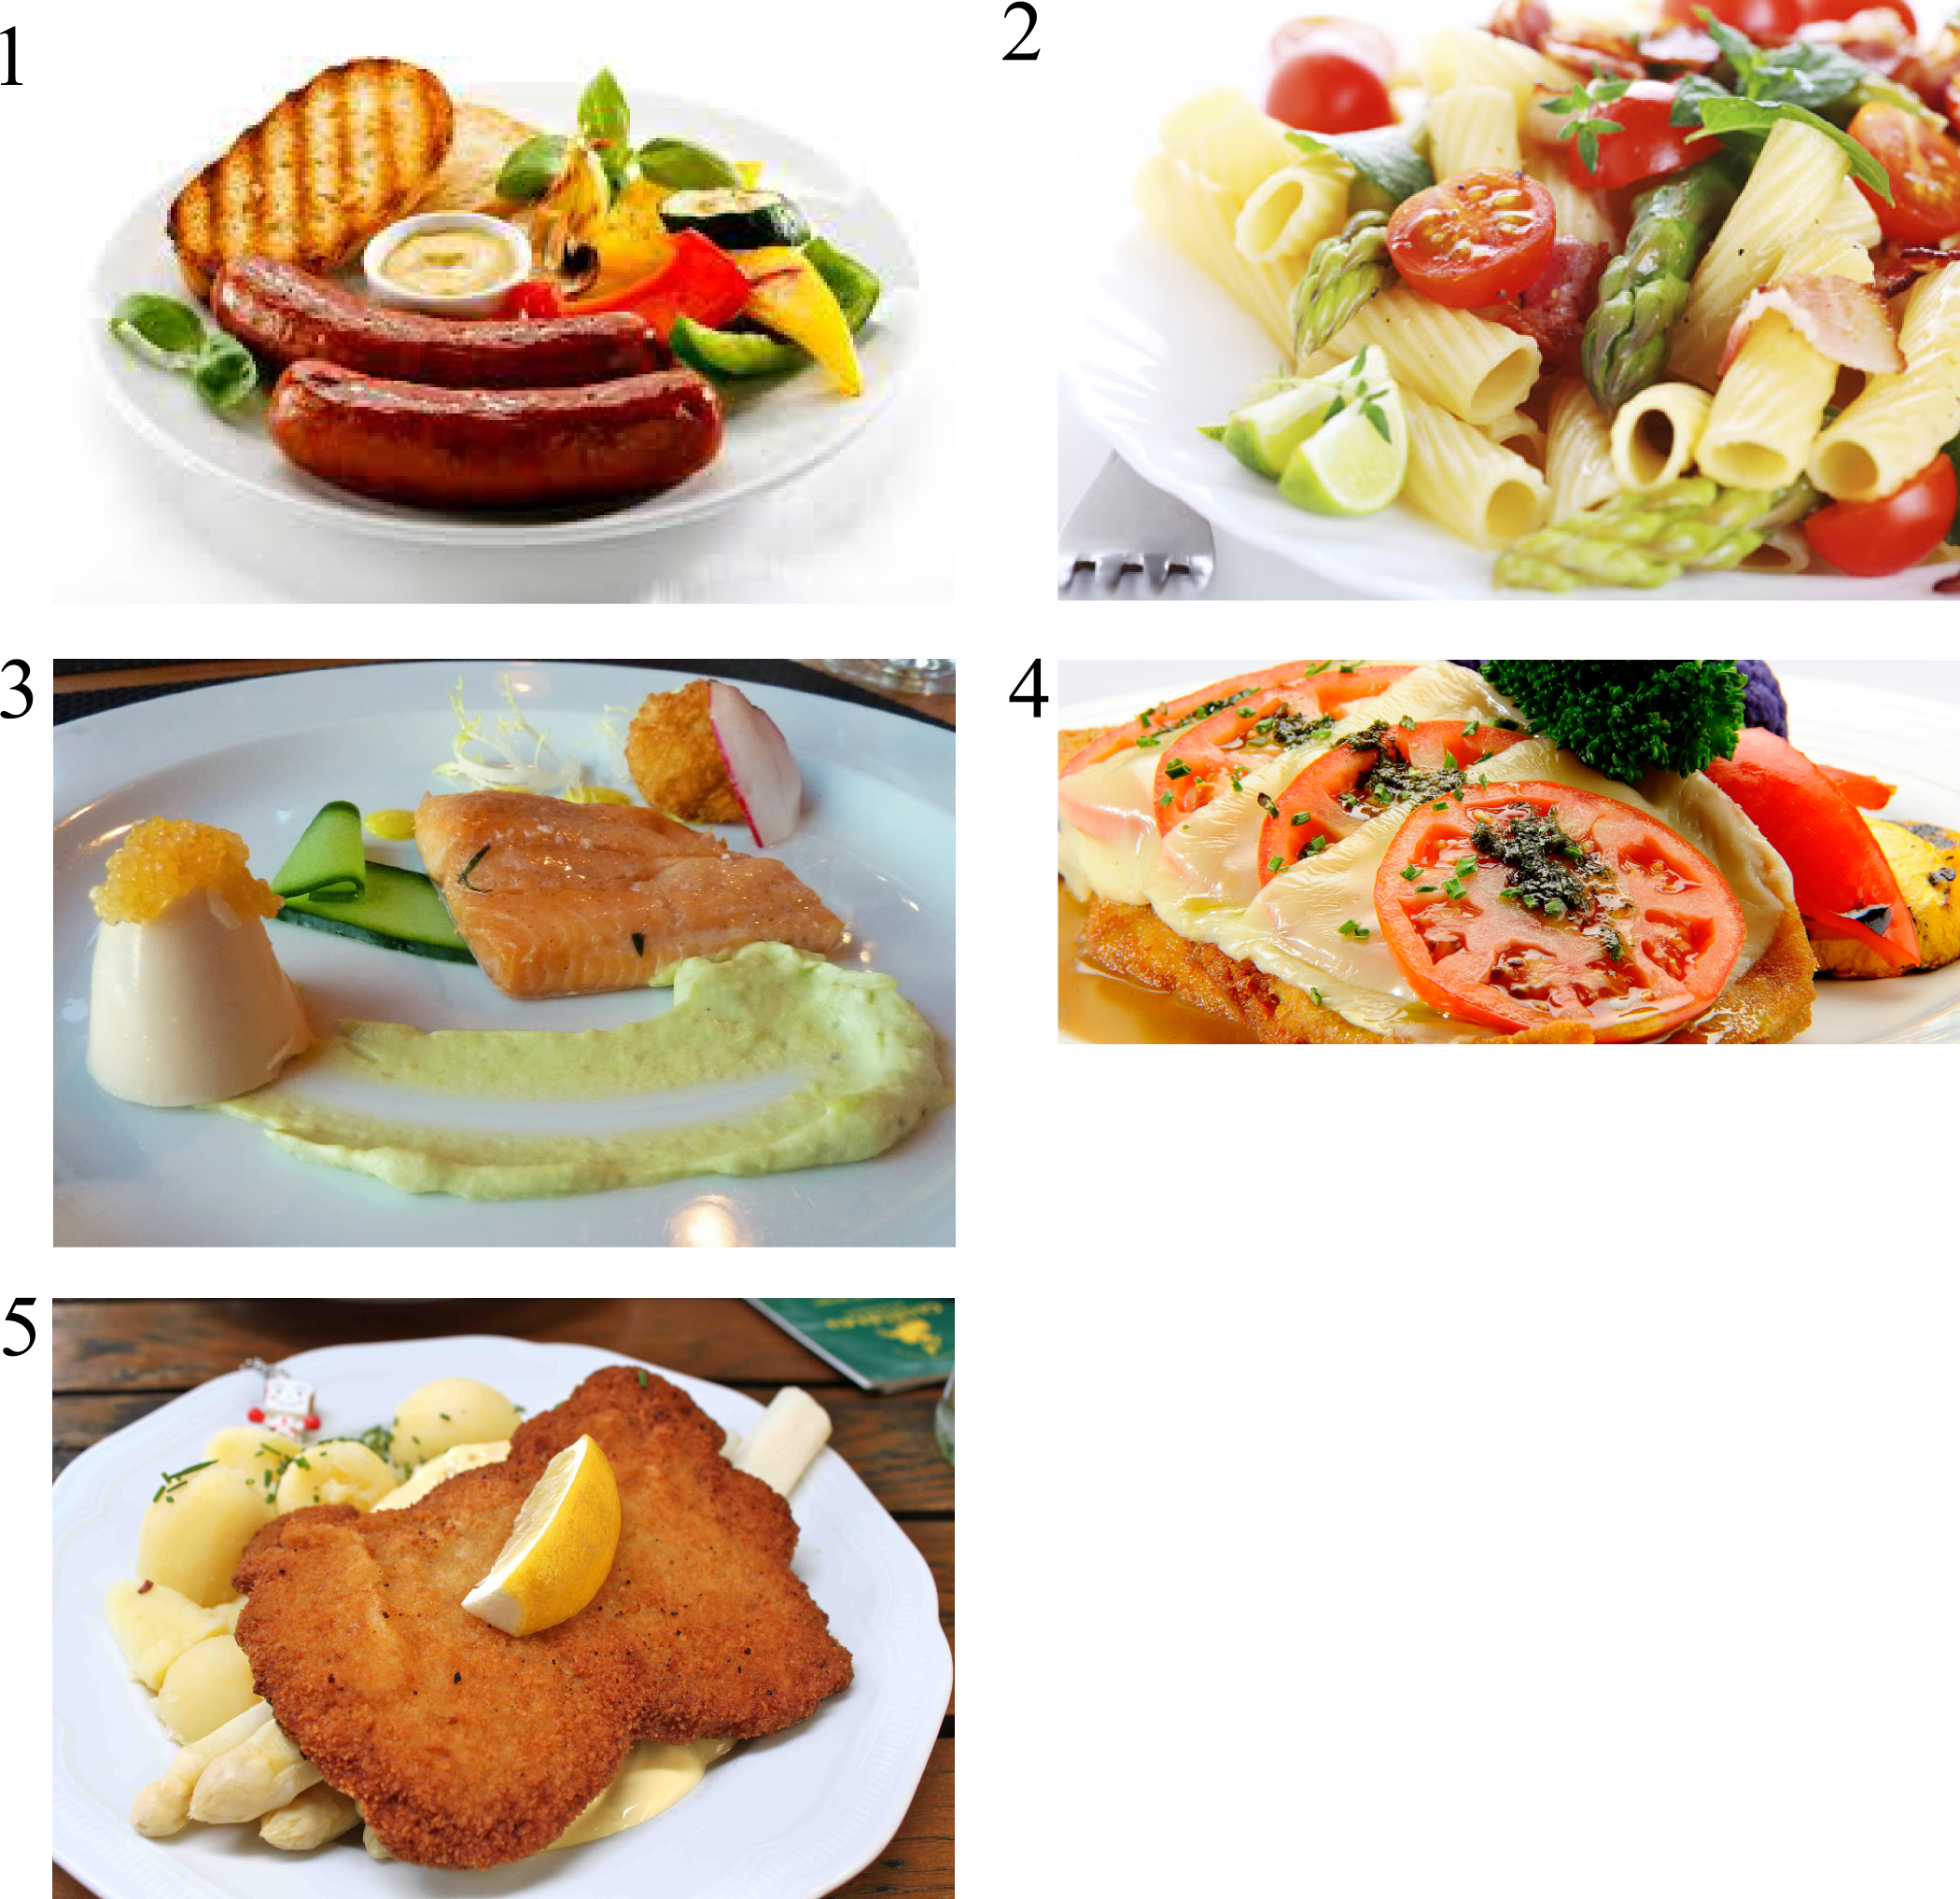
\includegraphics[scale=1.00]{../figs/ambiguous.png}
	\caption{caption here}
	\label{fig:ambiguous}
\end{figure*}

\begin{figure*}
%	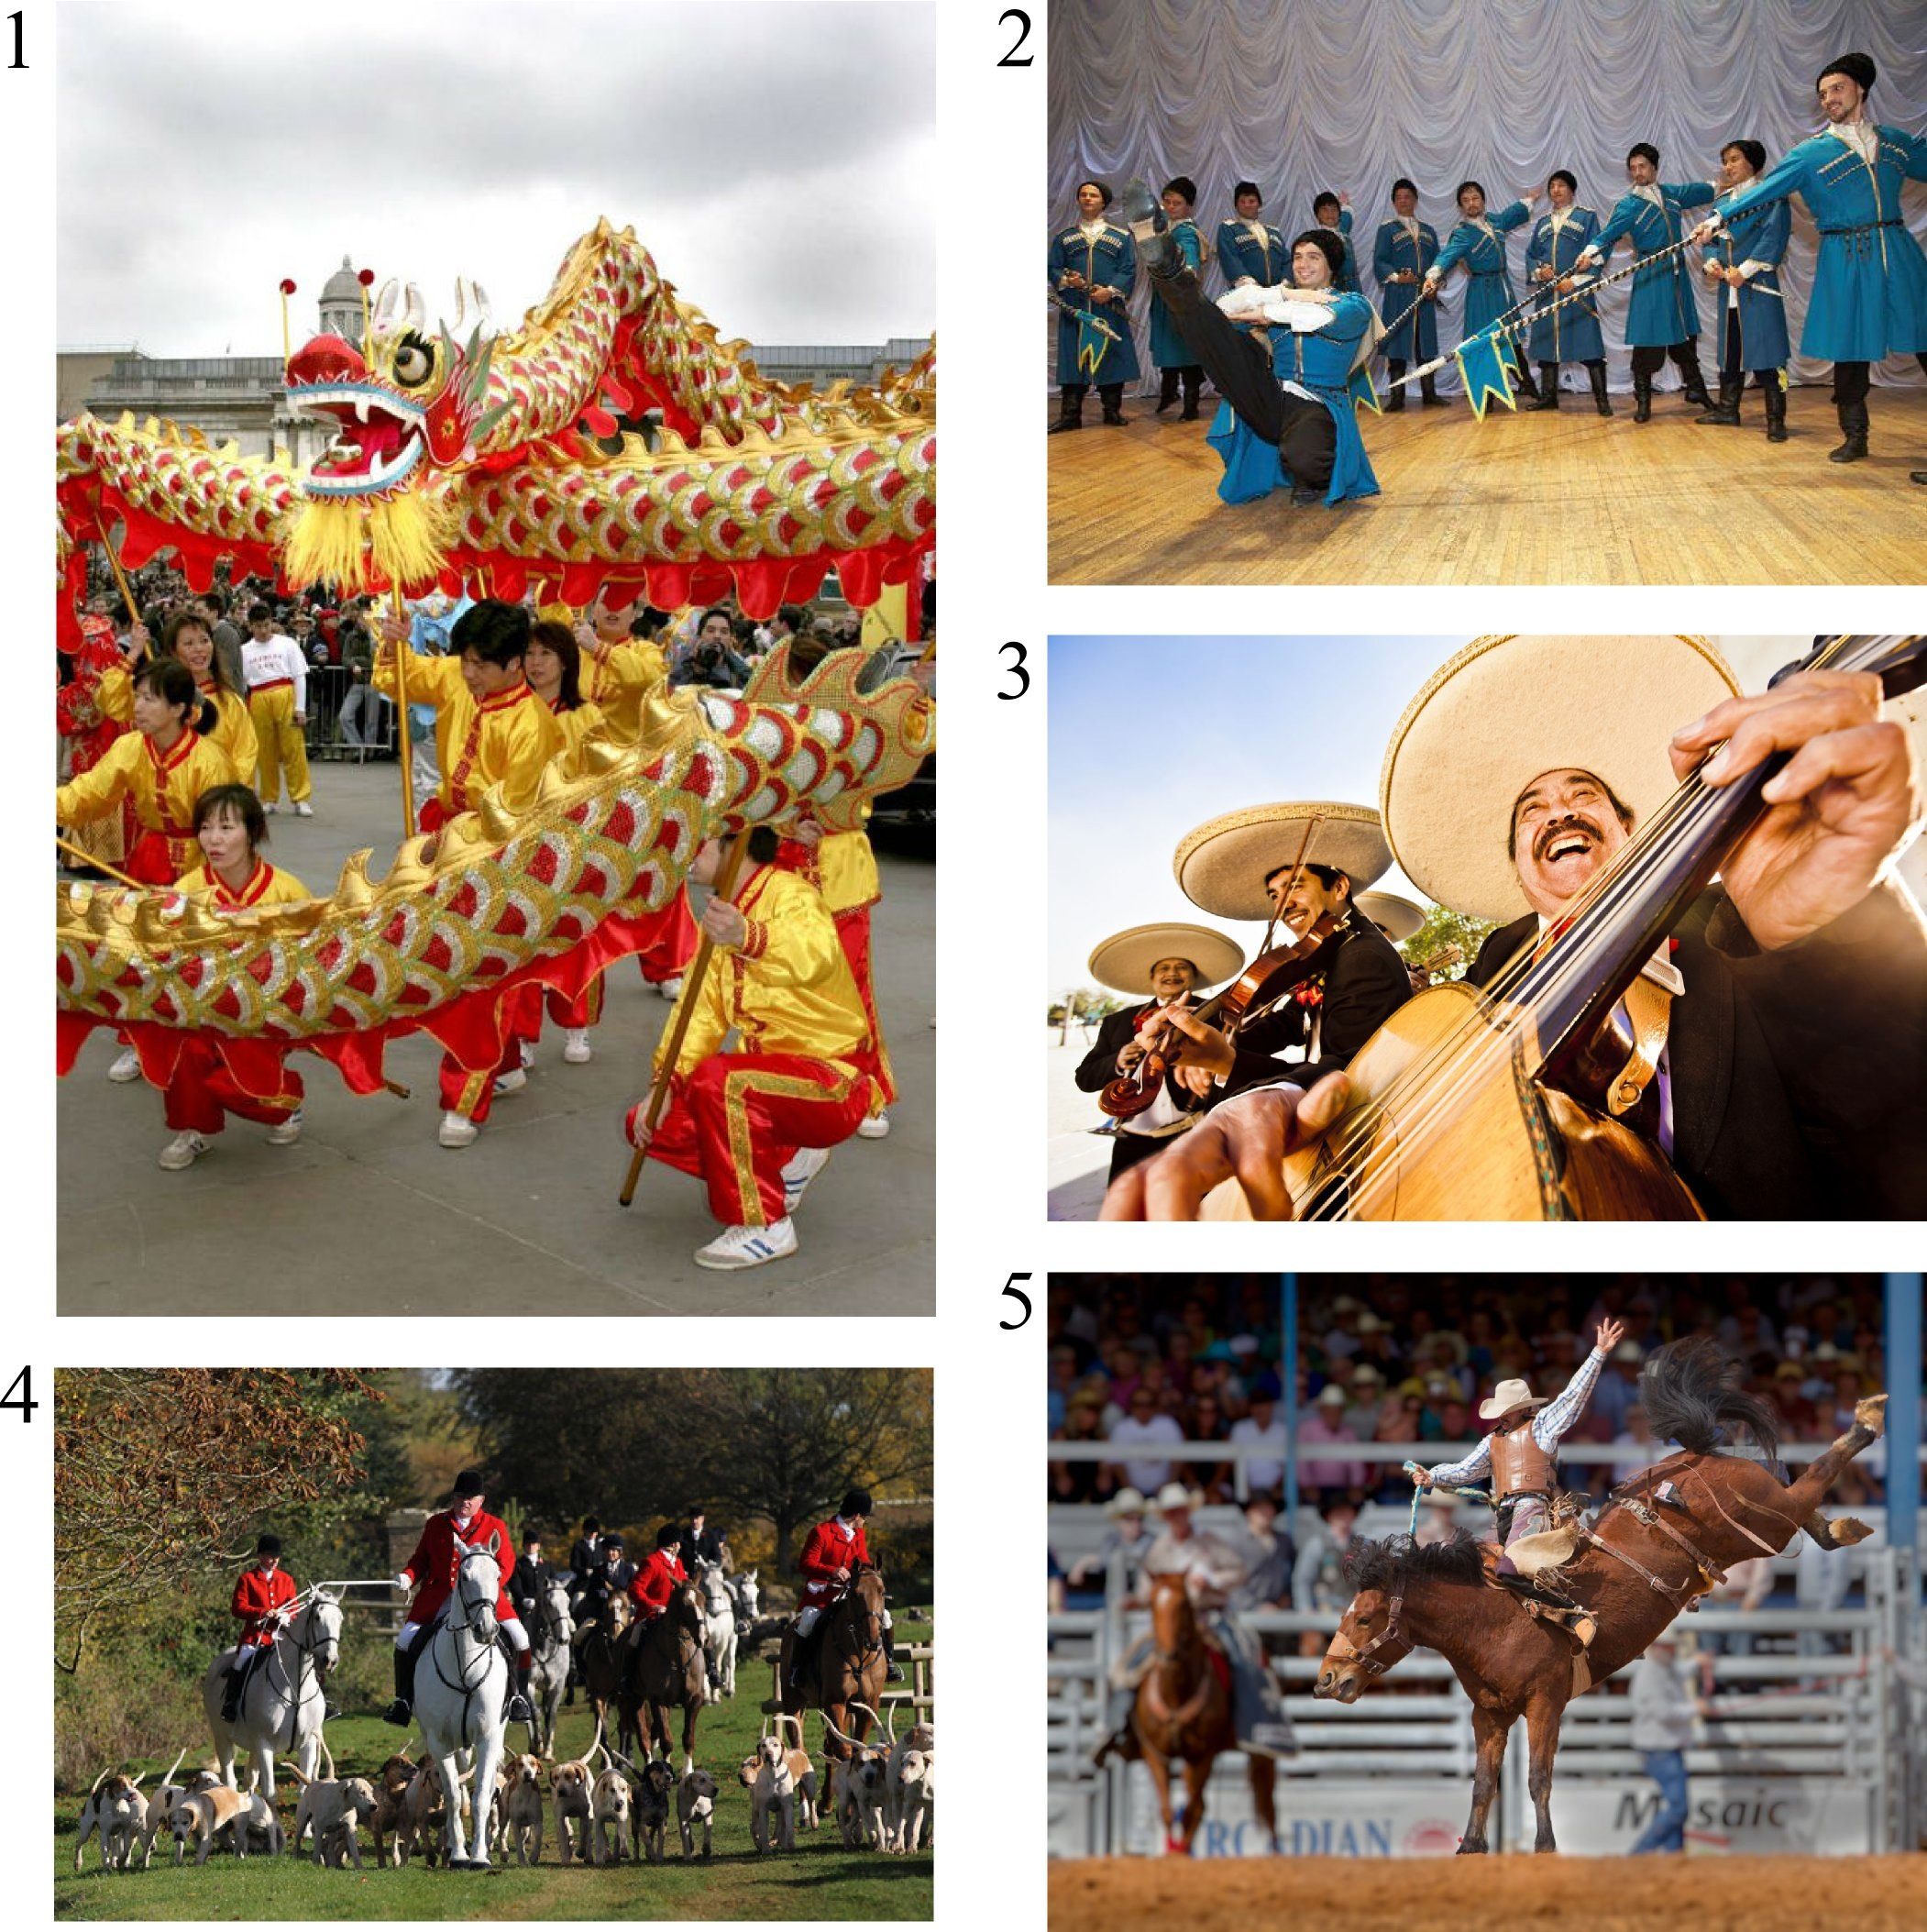
\includegraphics[scale=1.00]{../figs/cultural.png}
	\caption{caption here}
	\label{fig:cultural}
\end{figure*}

\begin{figure*}
%	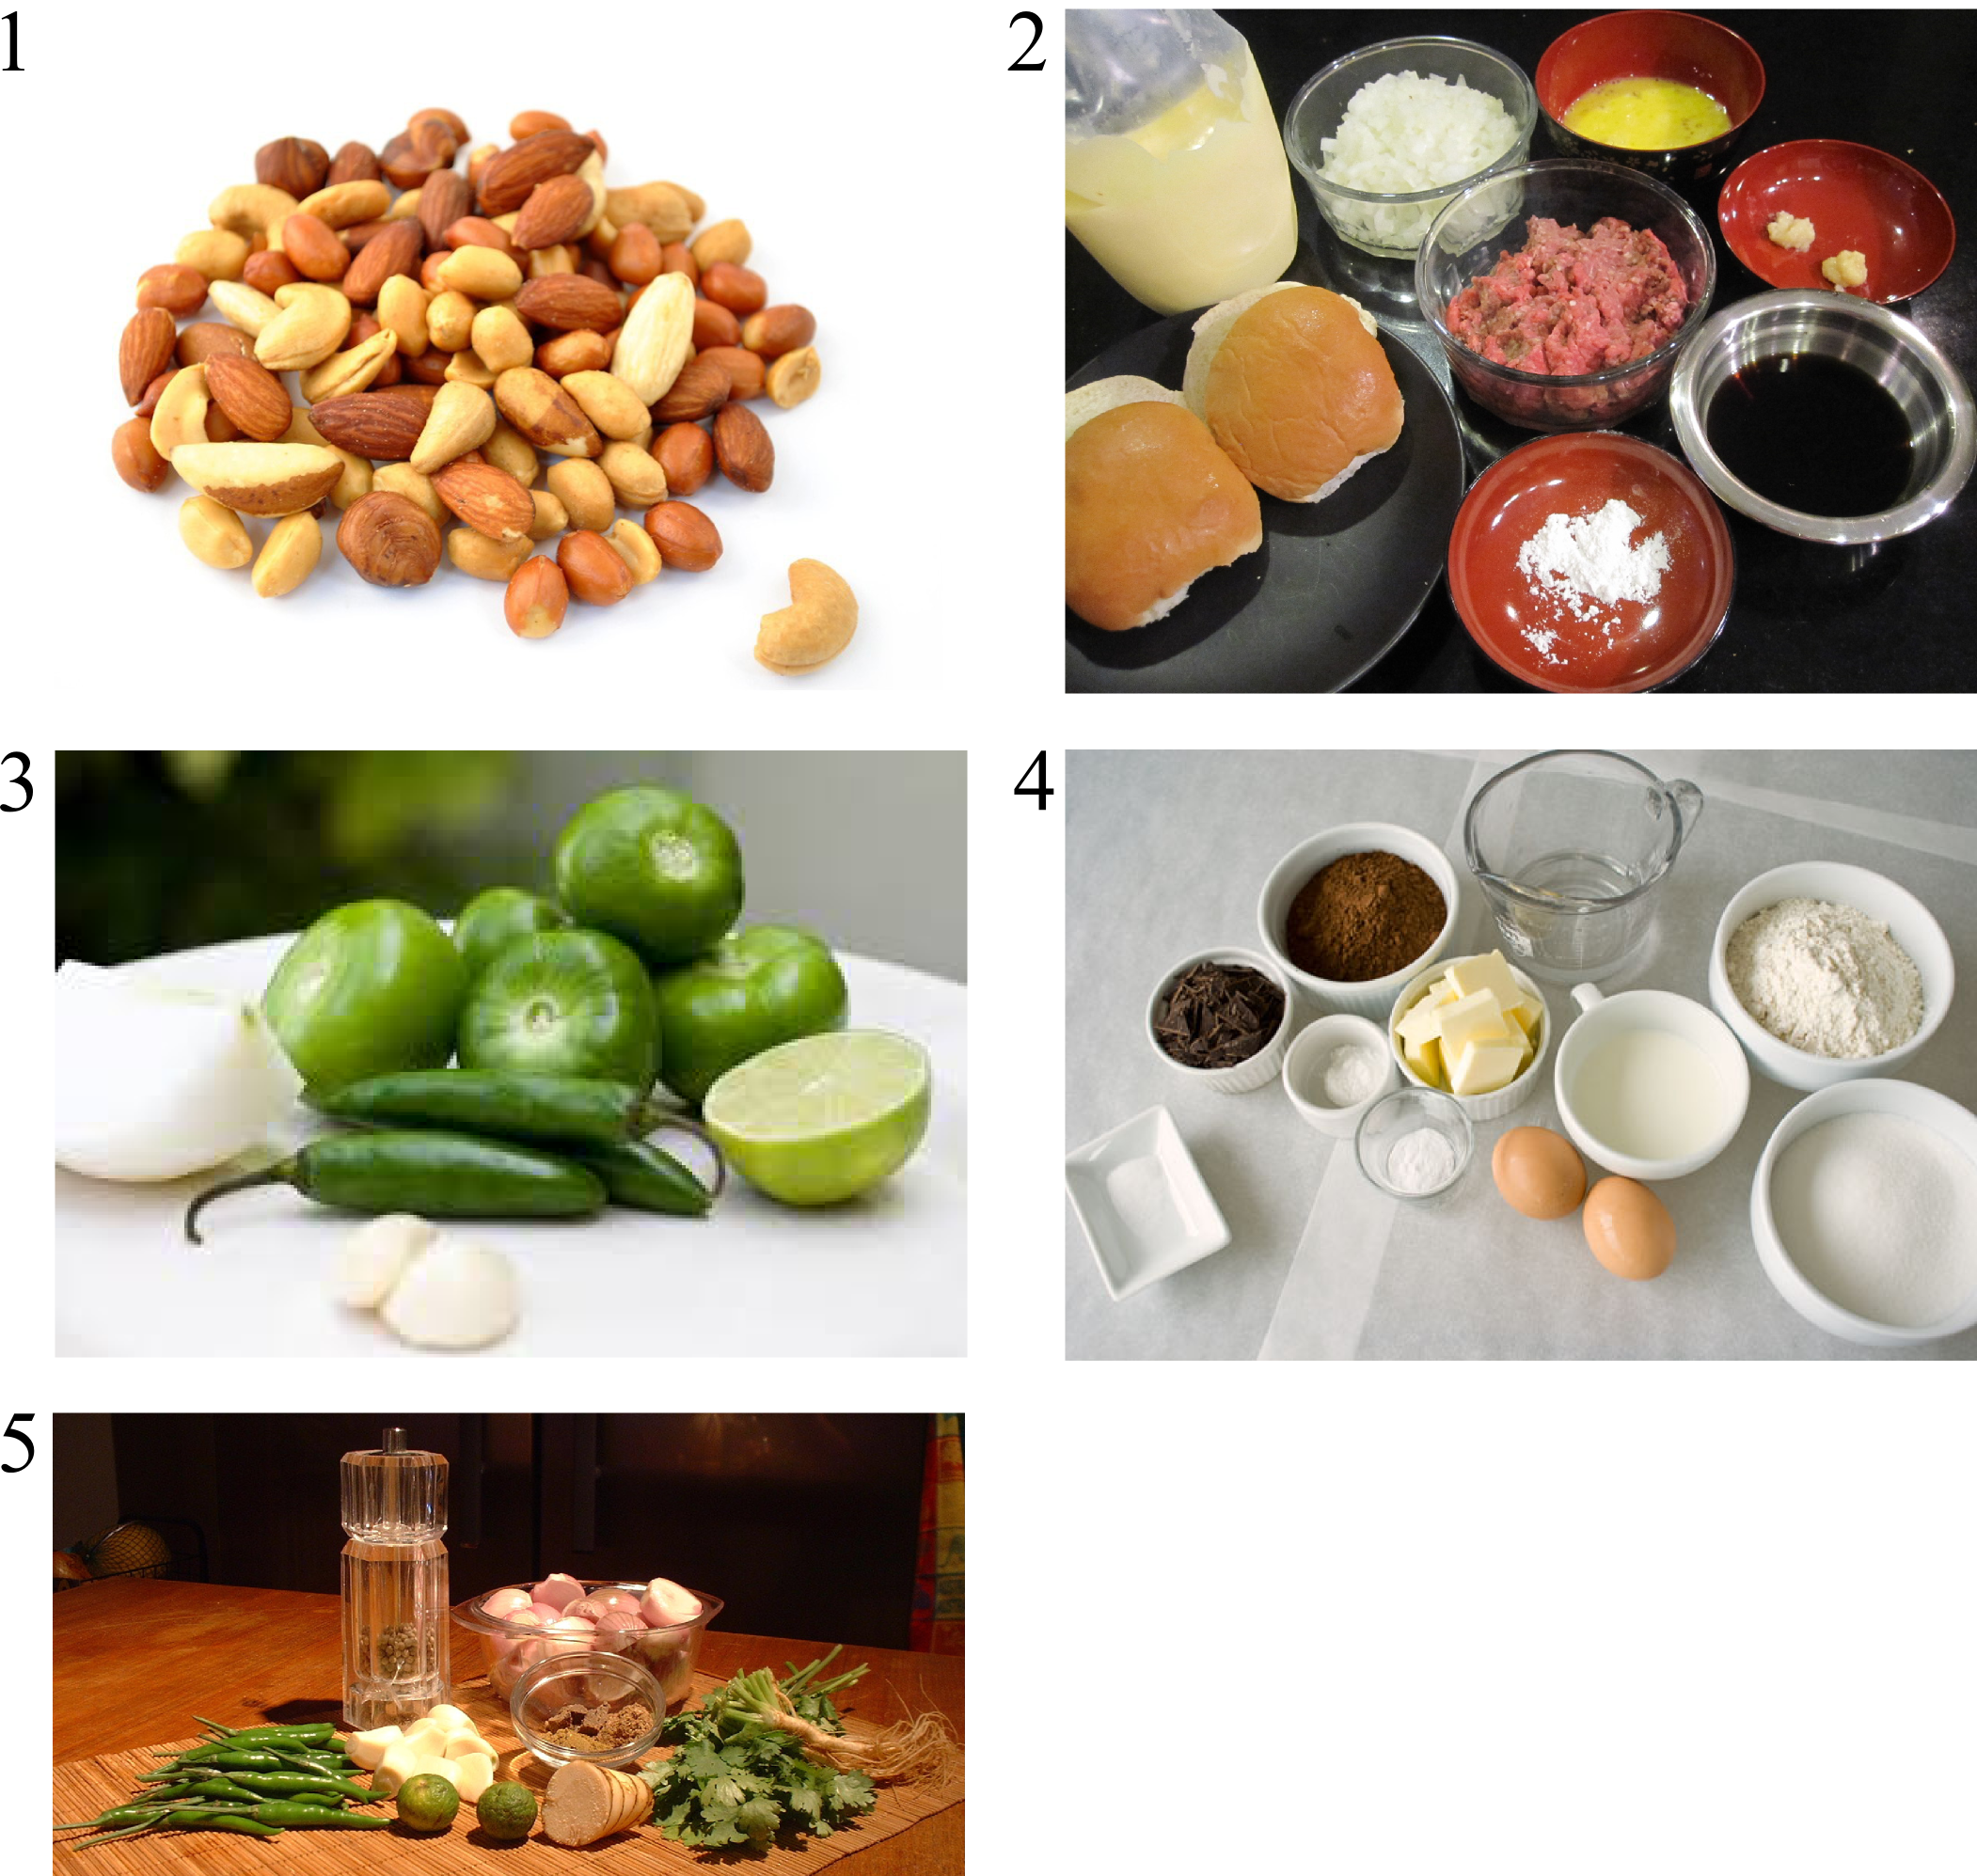
\includegraphics[scale=1.00]{../figs/ingredients.png}
	\caption{caption here}
	\label{fig:ingredients}
\end{figure*}

\bibliographystyle{plain}
\bibliography{bab.bib}
\end{document}
